\documentclass[a4paper,11pt]{article}
\usepackage[T1]{fontenc}
\usepackage{geometry}
\usepackage{fancyhdr}
\usepackage{tcolorbox}
\usepackage{multicol}
\usepackage{array}
\usepackage{tabularx}
\usepackage[table,xcdraw]{xcolor}
\usepackage{titlesec}
\usepackage{xcolor}

\usepackage{tikz}
\usepackage{forest}

\usepackage{hyperref}
\usepackage{amsmath}

\geometry{margin=2cm}

% Define custom column types with relative widths
\newcolumntype{L}[1]{>{\raggedright\arraybackslash\ttfamily}p{#1\linewidth}}
\newcolumntype{M}[1]{>{\raggedright\arraybackslash}p{#1\linewidth}}
\newcolumntype{R}[1]{>{\centering\arraybackslash}p{#1\linewidth}}

% Header and Footer
\pagestyle{fancy}
\fancyhead[L]{\textbf{GPUI Framework}}
\fancyhead[C]{Manual}
\fancyhead[R]{v1.0}
\fancyfoot[L]{\texttt{https://github.com/SvenSZim/GPUI}}
\fancyfoot[C]{}
\fancyfoot[R]{\thepage}
\usepackage{titlesec}

% Set section font size to 16pt
\titleformat{\section}[block]{\normalfont\LARGE\bfseries}{\thesection}{1em}{}
\titleformat{\subsection}[block]{\normalfont\Large\bfseries}{\thesubsection}{1em}{}
\titleformat{\subsubsection}[block]{\normalfont\large\bfseries}{\thesubsection}{1em}{}

% Link format
\hypersetup{
    colorlinks=true,
    linkcolor=black,
    urlcolor=gray,
    pdfborder={0 0 0}
}

\begin{document}
\title{General Purpose User Interface - GPUI}
\maketitle
The GPUI (General Purpose UI) framework is designed to let developers build flexible, composable user interfaces with a small set of well-defined primitives. Its goals are:

\begin{itemize}
    \item Simplicity: provide a concise API (XML + runtime) for declaring layouts and behaviour.
    \item Composability: make it easy to assemble complex widgets from small elements (boxes, lines, text, framed wrappers, groups).
    \item Reusability: support prefabs/styles so visual appearance and structure can be reused and swapped without changing layout logic.
    \item Predictability: explicit child/slot semantics and predictable layout rules so UIs behave consistently across different resolutions.
\end{itemize}
Who should use GPUI:

\begin{itemize}
    \item Game developers or lightweight app authors who want a small, deterministic UI system layered on a renderer.
    \item People who prefer layout-by-declaration (XML-style prefabs) with runtime access to named elements.
\end{itemize}
What to expect from this manual:

\begin{itemize}
    \item A reference of available XML elements and their attributes
    \item Clear guidance on what children each element accepts and how they are used
    \item Examples showing typical composition patterns and common use-cases
\end{itemize}

\section*{Basic example}
\vspace{-1.2em}
\rule{\linewidth}{0.4pt}
The smallest useful GPUI layout is a `UI` that contains a single panel with a button. Below is a minimal XML example demonstrating element composition and child usage (the button wraps a `text` child to provide its label):

\begin{verbatim}
<ui>
    <box label="mainpanel" colors="(40,40,48)" inset="12">
        <group spacing="8">
            <button onclick="sayHello" inset="10">
                <text color="white">Click me</text>
            </button>
            <text color="(200,200,200)" fontsize="m">Status: idle</text>
        </group>
    </box>
</ui>
\end{verbatim}

Notes on the example:
\begin{itemize}
    \item The `button` contains a single `text` child that defines its normal appearance. You can add a second child to style the pressed state separately.
    \item The `group` arranges children vertically by default and manages spacing between them.
    \item The `ui` root registers named elements (like `mainpanel`) for programmatic lookup at runtime.
\end{itemize}




\section*{Advanced use}
\vspace{-1.2em}
\rule{\linewidth}{0.4pt}
The \textbf{GPUI} (General Purpose UI) is built around modular units called \textbf{Elements}.  
Each Element encapsulates its \textbf{position}, \textbf{functionality}, \textbf{normal data}, and \textbf{render data}, which collectively define its behavior and appearance on the screen.

\begin{itemize}
    \item \textbf{Position} in GPUI is defined through \textit{joints}—dynamic relationships between elements. A joint links a relative position within one element to a relative position in another element (or to a static rectangle). Joints also support \textit{absolute offsets} in both x and y directions and can be used to \textit{fix the size} of elements similarly. This system enables flexible, constraint-based layout behavior.

    \item \textbf{Functionality} refers to the methods available to the element, such as subscribing to button events or responding to user input.

    \item \textbf{Normal data} represents element-specific content that isn’t exclusive to rendering—for example, the text in a text field.

    \item \textbf{Render data} includes appearance-related properties like font color, background color, and other visual attributes.
\end{itemize}

\subsection*{XML Parser}
\vspace{-1.2em}
\rule{\linewidth}{0.4pt}
GPUI uses \textbf{XML} to define and load layouts.

\hypertarget{tag}{}
\subsubsection*{Tags}

The \textbf{tag system} provides a shorthand for managing complex rendering logic. A tag is a named reference initialized with element-specific data, such as a color. Elements can then refer to these tags for rendering purposes—for example, using a tag-based \textit{color order} to alternate line segment colors in a \texttt{Line} element.

Tags must be strings that \textbf{do not start with a number} and \textbf{cannot contain} the characters: \texttt{=}, \texttt{:}, \texttt{;}, \texttt{[}, \texttt{]}, \texttt{\{}, or \texttt{\}}.

\subsection*{Event System}
\vspace{-1.2em}
\rule{\linewidth}{0.4pt}
GPUI includes a lightweight event system used to decouple user interaction (clicks, changes, drags) from application logic. Events are simple named signals that can carry a small payload (context) and are dispatched by elements or emitted programmatically.

Key concepts:
\begin{itemize}
    \item \textbf{Event names:} Events are identified by string names (for example, "myEvent" or "volumeChange"). Many element attributes (like \texttt{onclick}, \texttt{onchange}) are simply event names that the parser wires to the element's interaction hooks.
    \item \textbf{EventManager:} A central registry that manages subscriptions. Handlers can subscribe to event names and will be invoked whenever an event with that name is emitted.
    \item \textbf{Event payload:} Emitted events typically include a small payload object containing at least the event source (the element that fired the event) and any relevant data (new value, state, metadata). Handlers should expect a compact object/dict and avoid heavy data copies.
    \item \textbf{Local vs global triggers:} Some elements can be configured to emit events only when interacted with locally (inside their bounds) or as global triggers that respond regardless of focus or pointer position. Use the element's attributes to control this behaviour.
\end{itemize}

Common interaction mappings:
\begin{itemize}
    \item \texttt{Button}: emits the event named by \texttt{onclick} when pressed (and optionally during hold/release depending on configuration).
    \item \texttt{Toggle/Checkbox}: emits \texttt{onchange} when the state cycles/changes.
    \item \texttt{Slider}: emits \texttt{onchange} when the value changes (continuous or on-release depending on \texttt{step} and implementation).
\end{itemize}

Minimal usage examples:

XML (declarative):
\begin{verbatim}
<button onclick="myEvent">Click me</button>
<slider onchange="volumeChanged" />
\end{verbatim}

Python (subscribe at runtime):
\begin{verbatim}
from ui.interaction.event.eventmanager import EventManager

def on_my_event(evt):
    # evt is a small object/dict with at least: name, source, data
    print('Received', evt.name, 'from', evt.source)

EventManager.subscribe('myEvent', on_my_event)

# Emit programmatically (optional)
EventManager.emit('myEvent', {'value': 123})
\end{verbatim}

Best practices and notes:
\begin{itemize}
    \item Prefer simple payloads (primitives or small dicts) to avoid expensive copies across subscribers.
    \item Unsubscribe handlers when they are no longer needed (for example, when a screen or element is destroyed) to avoid memory leaks.
    \item Use unique, descriptive event names (e.g., \texttt{settings.audio.mute}) to reduce accidental collisions in large projects.
    \item For high-frequency events (drag/continuous slider updates) consider throttling or debouncing on the application side.
\end{itemize}

API hooks (common operations):
\begin{itemize}
    \item \texttt{EventManager.subscribe(name, handler)} — register a handler for an event name.
    \item \texttt{EventManager.unsubscribe(name, handler)} — remove a previously-registered handler.
    \item \texttt{EventManager.emit(name, payload)} — emit a named event with an optional payload.
    \item Element attributes like \texttt{onclick} / \texttt{onchange} — declarative wiring from XML to event names.
\end{itemize}

This event system keeps UI code concise and makes it easy to connect declarative XML layouts to application logic without tight coupling.


\newpage
\subsection*{Available XML-Elements}
\vspace{-1.2em}
\rule{\linewidth}{0.4pt}


\hypertarget{line}{}
\subsubsection*{Line-Element}
The \texttt{Line}-Element is used to specify a line to be drawn in the UI.
\begin{center}
    \texttt{<line>} | \texttt{<l>}
\end{center}

\renewcommand{\arraystretch}{1.3}
\begin{tcolorbox}[colback=white, colframe=black!75, title=Arguments]
\begin{tabularx}{\linewidth}{p{45pt}|p{90pt}|X}
\textbf{Name} & \textbf{Values} & \textbf{Description}\\
\hline
colors/ color/ col & tag:color;... & Defines tag-based colors for lines. Values can be RGB (r,g,b) or color names (e.g., "red"). "inv"/"none" makes them invisible. If no tag is set (e.g., "color=red"), default tag '' is used. Default: inv\\
\rowcolor[HTML]{E8E8E8}
flip & & Draws line from bottom-left to top-right instead of default top-left to bottom-right. Default: noflip\\
inset & float|float,float| int|int,int & Adds padding to the line. One value applies to both dimensions; two values set width and height separately. Ints are absolute; floats are percentages. Default: 0\\
\rowcolor[HTML]{E8E8E8}
order/ sectionorder & tag1,tag2,... & Specifies a sequence of tags for color/size/thickness, repeated cyclically along the line. Default: '' (default tag)\\
sizes/ size & tag:float|int;... & Sets segment lengths (absolute or relative) per tag. Uses default tag '' if unspecified. Default: 1.0\\
\rowcolor[HTML]{E8E8E8}
thickness/ width & tag:int;... & Sets absolute line thickness per tag. Uses default tag '' if unspecified. Default: 1\\
& EXPERIMENTAL & \\
\rowcolor[HTML]{E8E8E8}
altmode & tag:mode;... & Alternate drawing mode. Supported: cross. Default: default
\end{tabularx}
\end{tcolorbox}

\begin{minipage}{0.35\linewidth}
Example (256×144):\\
<line\\color="inv;r:red;b:blue;w:white"\\thickness="1;b:2;w:3"\\flip=""\\sizes="10;r:0.15;b:0.20;w:5"\\inset="25"\\sectionorder="r,,w,,b,"\\altmode="r:cross">
</line>
\end{minipage}
\hfill
\begin{minipage}{0.55\linewidth}
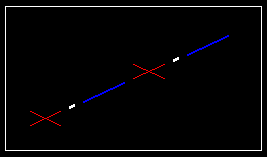
\includegraphics[width=\linewidth]{images/line.png}
\end{minipage}


\newpage
\hypertarget{box}{}
\subsubsection*{Box-Element}
The \texttt{Box}-Element is used to specify a box to be drawn in the UI.
\begin{center}
    \texttt{<box>} | \texttt{<b>}
\end{center}

\renewcommand{\arraystretch}{1.3}
\begin{tcolorbox}[colback=white, colframe=black!75, title=Arguments]
\begin{tabularx}{\linewidth}{p{60pt}|p{110pt}|X}
\textbf{Name} & \textbf{Values} & \textbf{Description}\\
\hline
colors/ color/ col & tag:color;... & Defines tag-based colors for rendering. Colors can be RGB tuples (r,g,b) or names (e.g., "red"). "inv" or "none" make elements invisible. If no tag is specified (e.g., "color=red"), the default tag '' is used. Default: inv\\
\rowcolor[HTML]{E8E8E8}
fillmode(s)/ fill(s)/ altmode(s)/ mode(s) & tag:mode;... & Sets the fill pattern for sub-boxes: striped vertically/horizontally or checkerboard. Values: striped\_vert (strv), striped\_hor (strh), checkerboard (cb). Uses default tag '' if none given. Default: solid\\
fillsize(s)/ innersizing(s)/ size(s) & tag:int|float;... & Sets size of the alternating pattern, either absolute or relative. Uses default tag '' if none given. Default: 10\\
\rowcolor[HTML]{E8E8E8}
inset & float|float,float| int|int,int & Sets padding inside the box. One value applies to both dimensions; two values specify width and height separately. Ints are absolute; floats are percentages. Default: 0\\
orders/ sectionorders/ ord & tag:tag1,tag2,...;... & Defines tag sequence used to render fill patterns cyclically in sub-boxes. Uses default tag '' if none given. Default: ''\\
\rowcolor[HTML]{E8E8E8}
partitioning/ part & intxint;[c1,c2,...]| [1=c1,3=c3,...]| 4=[...] & Splits the box into columns × rows of sub-boxes. Each sub-box can have its own fillmode, size, and filter defined by tags. Labels are set per row or column using square brackets. Sub-boxes have ''-tag per default. Default: 1x1\\
& EXPERIMENTAL & \\
\rowcolor[HTML]{E8E8E8}
filter(s)/ filt & tag:mode= float,float,float+float;... & Applies shape filters to sub-boxes. Modes: triangle/linear/quadratic/circle, with optional inversion ("i" prefix). Filters define a point and max distance for visible area. Default: nofilter
\end{tabularx}
\end{tcolorbox}

\begin{minipage}{0.35\linewidth}
Example (960×560):\\
    <box\\partitioning="4x2;[a,b,a,b][2=c,4=c]"\\filter="b:it=0.5,0.0,0.5+0.0"\\inset="80"\\colors=\\"(240,30,30);c1:(120,30,30);c2:(60,60,60)"\\fillmode="a:strh;b:cb;c:strv"\\fillsize="40"\\sectionorders=\\"c3;a:c1,c2;b:c1,c2;c:c1,c2"></box>
\end{minipage}
\hfill
\begin{minipage}{0.55\linewidth}
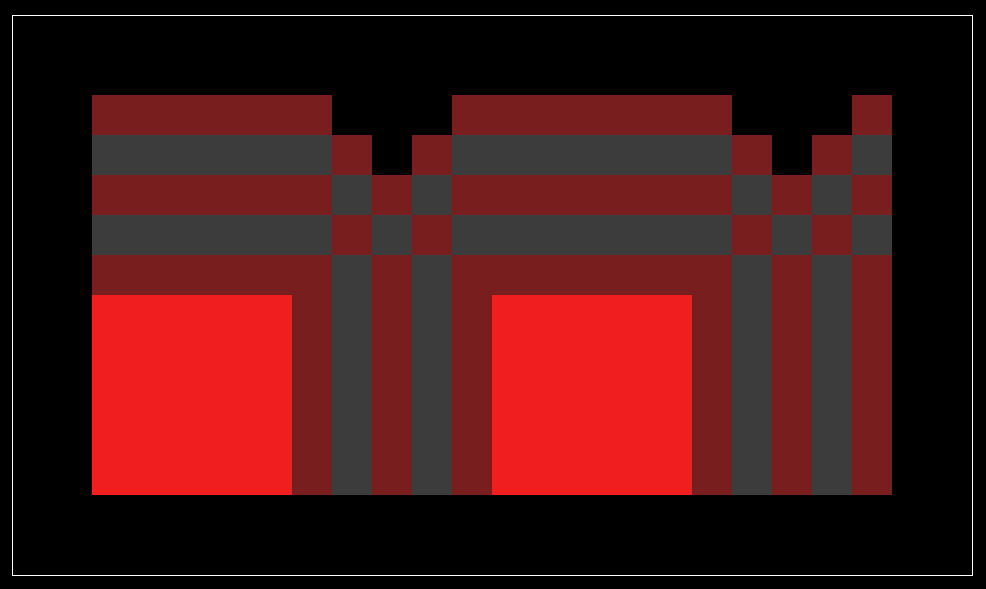
\includegraphics[width=\linewidth]{images/box.png}
\end{minipage}


\newpage
\hypertarget{text}{}
\subsubsection*{Text-Element}
The \texttt{Text}-Element is used to specify a text to be drawn in the UI.
\begin{center}
    \texttt{<text>} | \texttt{<t>}
\end{center}

\renewcommand{\arraystretch}{1.3}
\begin{tcolorbox}[colback=white, colframe=black!75, title=Arguments]
\begin{tabularx}{\linewidth}{p{50pt}|p{110pt}|X}
\textbf{Name} & \textbf{Values} & \textbf{Description}\\
\hline
align & float|l|r,float|t|b & Sets the align of the text inside the text-box. Default: 0.5,0.5\\
\rowcolor[HTML]{E8E8E8}
colors/ color/ col & color & Defines fontcolor for rendering. Color can be RGB tuple (r,g,b) or name (e.g., "red"). "inv" or "none" makes text invisible. Default: inv\\
fontname/ sysfont/ font & fontname;... & Sets font for rendering . Default: Arial\\
\rowcolor[HTML]{E8E8E8}
fontsize/ size & d|int|xxs|xs|...|xl|xxl;... & Sets fontsize for rendering. 'd' sets the fontsize to be dynamicly calculated. Default: 24\\
inset & float|float,float| int|int,int & Sets padding inside the box. One value applies to both dimensions; two values specify width and height separately. Ints are absolute; floats are percentages. Default: 0\\
\end{tabularx}
\end{tcolorbox}

\begin{minipage}{0.35\linewidth}
Example (640×360):\\
      <text\\inset="100"\\color="red"\\fontsize="l"\\align="0.3,0.9">\\Hello World\\</text>
\end{minipage}
\hfill
\begin{minipage}{0.55\linewidth}
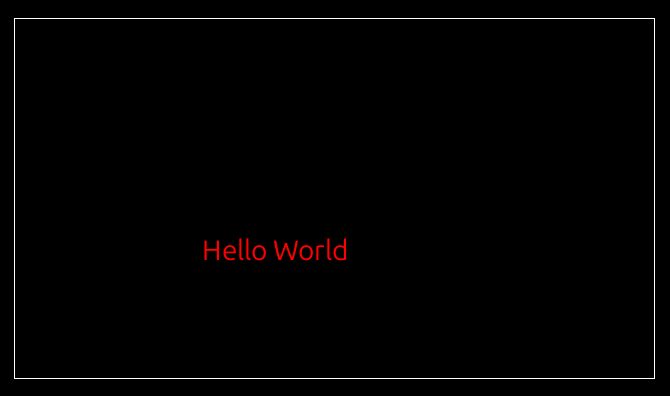
\includegraphics[width=\linewidth]{images/text.png}
\end{minipage}



\newpage
\hypertarget{framed}{}
\subsubsection*{Framed-Element}
The \texttt{Framed}-Element provides a flexible container that enhances elements with customizable borders and backgrounds. It supports individual border styling for each edge and optional background elements with advanced visual effects.
\begin{center}
    \texttt{<framed>} | \texttt{<fr> | \texttt{<f>}}
\end{center}

\renewcommand{\arraystretch}{1.3}
\begin{tcolorbox}[colback=white, colframe=black!75, title=Arguments]
\begin{tabularx}{\linewidth}{p{50pt}|p{110pt}|X}
\textbf{Name} & \textbf{Values} & \textbf{Description}\\
\hline
inset/ offset/ padding & int & Sets padding inside the box. Default: 0\\
\end{tabularx}
\end{tcolorbox}

\renewcommand{\arraystretch}{1.3}
\begin{tcolorbox}[colback=white, colframe=black!75, title=Children]
\begin{tabularx}{\linewidth}{p{50pt}|p{110pt}|X}
\textbf{Name} & \textbf{Amount} & \textbf{Description}\\
\hline
\hyperlink{line}{\texttt{Line}} & 0 - 4 & Sets the borders of the framed. If one is provided it is applied to all sides. If two are provided, the first is applied to left and right and the second to top and bottom. Otherwise borders are applied like 1-left, 2-right, 3-top, 4-bottom. Default: noborders\\
\rowcolor[HTML]{E8E8E8}
\hyperlink{box}{\texttt{Box}} & 0 - 1 & Sets the background of the framed. Default: nobackground\\
\texttt{Any Element} & 1 & Wrapped element.\\
\end{tabularx}
\end{tcolorbox}

Example (640×360):\\
<framed offset="50">\\
  <line color="inv;r:red" thickness="3" sizes="10;n:20" inset="0.1" sectionorder="r,n"></line>\\
  <line color="white"></line>\\
  <line color="inv;r:red" thickness="3" sizes="10;n:20" inset="0.1" sectionorder="r,n"></line>\\
  <box colors="(0,0,240);a:(0,120,0)" inset="0.05" fillmode="strv" sectionorders=",a" filter="c=0.5,0.5,0.5+0.5" fillsize="15"></box>\\
  <text inset="50" color="(160,120,160)" fontsize="d">Hello World</text>\\
</framed>
\begin{figure}[h]
    \centering
    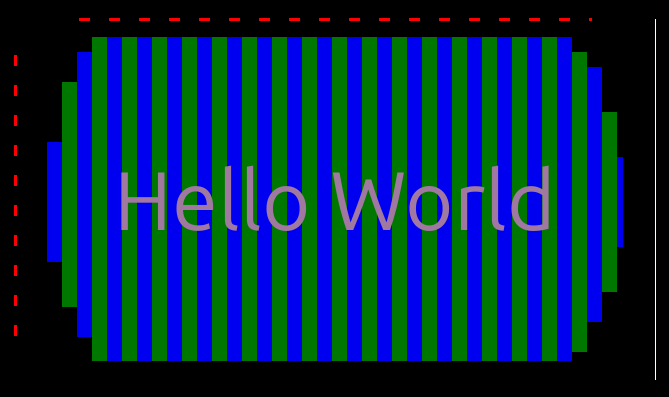
\includegraphics[width=0.5\linewidth]{images/framed.png}
\end{figure}



\newpage
\hypertarget{group}{}
\subsubsection*{Group-Element}
The \texttt{Group}-Element provides a powerful layout organization system that arranges multiple elements in vertical or horizontal configurations. Groups handle automatic sizing, spacing, and alignment while supporting nested grouping for complex layouts.
\begin{center}
    \texttt{<group>} | \texttt{<group>} | \texttt{<gr> | \texttt{<g>}}
\end{center}

\renewcommand{\arraystretch}{1.3}
\begin{tcolorbox}[colback=white, colframe=black!75, title=Arguments]
\begin{tabularx}{\linewidth}{p{50pt}|p{110pt}|X}
\textbf{Name} & \textbf{Values} & \textbf{Description}\\
\hline
horizontal/ hor & & Sets the group to align the elements horizontal. Default: vertical\\
\rowcolor[HTML]{E8E8E8}
offset/ spacing & int & Sets the spacing between elements in the group. Default: 0\\
size(s)/ sizing(s) & float|int=float,... & Sets the relative sizing of the elements inside the group. Default: 1.0\\
\end{tabularx}
\end{tcolorbox}

\renewcommand{\arraystretch}{1.3}
\begin{tcolorbox}[colback=white, colframe=black!75, title=Children]
\begin{tabularx}{\linewidth}{p{50pt}|p{110pt}|X}
\textbf{Name} & \textbf{Amount} & \textbf{Description}\\
\hline
\texttt{Any Element} & 1+ & Grouped elements.\\
\end{tabularx}
\end{tcolorbox}

Example (640×360):\\
<group spacing="40" hor="" sizings="0.5,0.3,0.2">\\
<group spacing="20" sizing="2=1.4">\\
<box color="red"></box>\\
<box color="(160,0,0)"></box>\\
<box color="(80,0,0)"></box>\\
</group>\\
<box color="green"></box>\\
<box color="blue"></box>\\
</group>

\begin{figure}[h]
    \centering
    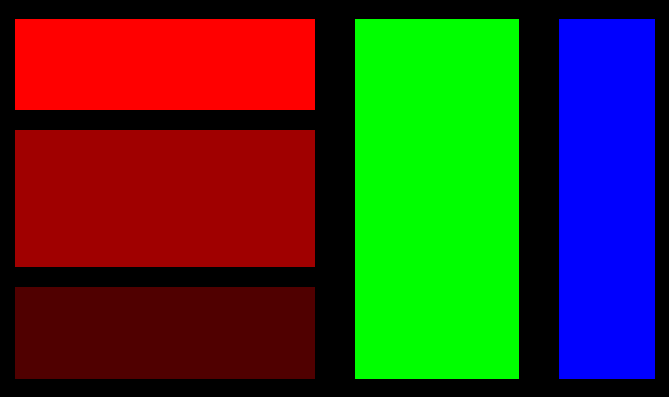
\includegraphics[width=0.5\linewidth]{images/group.png}
\end{figure}



\newpage
\hypertarget{dropdown}{}
\subsubsection*{Dropdown-Element}
The \texttt{Dropdown}-Element is used to create a dropdown.
\begin{center}
    \texttt{<dropdown>} | \texttt{<dpd>}
\end{center}

\renewcommand{\arraystretch}{1.3}
\begin{tcolorbox}[colback=white, colframe=black!75, title=Arguments]
\begin{tabularx}{\linewidth}{p{50pt}|p{110pt}|X}
\textbf{Name} & \textbf{Values} & \textbf{Description}\\
\hline
horizontal/ hor & & Sets the dropdown to be horizontal. Default: vertical\\
\rowcolor[HTML]{E8E8E8}
offset/ spacing & int & Sets the spacing between elements in the dropdown. Default: 0\\
size(s)/ sizing(s) & float|int=float,... & Sets the relative sizing of the elements inside the dropdown. Default: 1.0\\
\end{tabularx}
\end{tcolorbox}

\renewcommand{\arraystretch}{1.3}
\begin{tcolorbox}[colback=white, colframe=black!75, title=Children]
\begin{tabularx}{\linewidth}{p{50pt}|p{110pt}|X}
\textbf{Name} & \textbf{Amount} & \textbf{Description}\\
\hline
\texttt{Any Element} & 1+ & First element is the one to click to reveal the other elements as dropdown.\\
\end{tabularx}
\end{tcolorbox}

Example (128×72):\\
<dpd spacing="10" hor="" sizings="0.5,0.3,0.2,c5=1.2">\\
<box color="green"></box>\\
<dpd spacing="20" sizing="c2=1.9">\\
<box color="red"></box>\\
<box color="(160,0,0)"></box>\\
<box color="(80,0,0)"></box>\\
</dpd>\\
<box color="blue"></box>\\
<box color="green"></box>\\
<box color="blue"></box>\\
<box color="green"></box>\\
</dpd>

\begin{figure}[h]
    \centering
    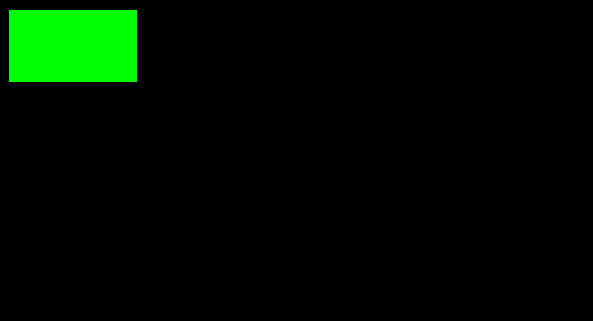
\includegraphics[width=0.45\linewidth]{images/dropdown1.png}
    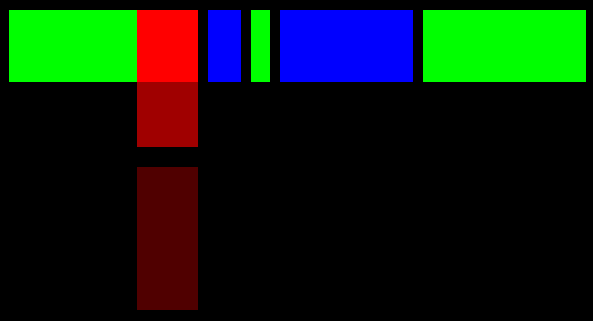
\includegraphics[width=0.45\linewidth]{images/dropdown2.png}
\end{figure}
\newpage
\hypertarget{button}{}
\subsubsection*{Button-Element}
The \texttt{Button}-Element provides an interactive clickable component with press, hold, and release states. It supports both local and global event triggering, and can be visually customized for different interaction states.
\begin{center}
        	\texttt{<button>} | \texttt{<btn>}
\end{center}

Buttons support several interaction modes:
\begin{itemize}
    \item Click events with optional hold-state tracking
    \item Global trigger events that work anywhere on screen
    \item Local trigger events that only work within button bounds
    \item Press and release state visualization
    \item Multiple callback subscription methods
\end{itemize}

\renewcommand{\arraystretch}{1.3}
\begin{tcolorbox}[colback=white, colframe=black!75, title=Arguments]
\begin{tabularx}{\linewidth}{p{60pt}|p{110pt}|X}
	\textbf{Name} & \textbf{Values} & \textbf{Description}\\
\hline
text/ content & string & Label text shown on the button. Default: ''\\
\rowcolor[HTML]{E8E8E8}
colors/ color & tag:color;... & Render colors for background/border/text using tag-based scheme (see Box/Text). Default: inv\\
onclick/ on & eventname & Event name to be fired when button is pressed (subscribe via EventManager). Default: none\\
\rowcolor[HTML]{E8E8E8}
inset & float|int & Padding inside the button. Default: 0\\
size/ sizing & float|int & Size hints. Default: dynamic\\
\end{tabularx}
\end{tcolorbox}

\renewcommand{\arraystretch}{1.3}
\begin{tcolorbox}[colback=white, colframe=black!75, title=Children]
\begin{tabularx}{\linewidth}{p{60pt}|p{110pt}|X}
	\textbf{Name} & \textbf{Amount} & \textbf{Description}\\
\hline
	\texttt{Any Element} & 0 - 2 & First element defines the unclicked state appearance, second (optional) defines the clicked state appearance. If only one element is provided, it's used for both states. If no elements are provided, default styling is used.\\
\end{tabularx}
\end{tcolorbox}

Example:\\
<button onclick="myEvent" inset="20">\\
<text color="white">Click me</text>\\
</button>

\newpage
\hypertarget{checkbox}{}
\subsubsection*{Checkbox / Toggle-Element}
The \texttt{Checkbox} or generic \texttt{Toggle}-Element provides boolean and multi-state toggles with customizable state transitions and visual feedback. Each state can have its own visual representation and trigger specific callbacks.
\begin{center}
        	\texttt{<checkbox>} | \texttt{<cycle>} | \texttt{<elementcycle>}
\end{center}

The Toggle system provides:
\begin{itemize}
    \item Multiple visual states with smooth transitions
    \item State-specific callback subscriptions
    \item Flexible state cycling patterns
    \item Global and local trigger events
    \item Optional hold-state behavior
\end{itemize}

\renewcommand{\arraystretch}{1.3}
\begin{tcolorbox}[colback=white, colframe=black!75, title=Arguments]
\begin{tabularx}{\linewidth}{p{60pt}|p{110pt}|X}
	\textbf{Name} & \textbf{Values} & \textbf{Description}\\
\hline
typ & checkbox|cycle & Type of toggle (checkbox = boolean, cycle = cycles through values). Default: checkbox\\
\rowcolor[HTML]{E8E8E8}
values & v1,v2,... & For cycle toggles, the sequence of states. Default: on,off\\
onchange & eventname & Event fired on state change.\\
\rowcolor[HTML]{E8E8E8}
colors & tag:color;... & Colors for each state; follows tag-based color scheme.\\
\end{tabularx}
\end{tcolorbox}

\renewcommand{\arraystretch}{1.3}
\begin{tcolorbox}[colback=white, colframe=black!75, title=Children]
\begin{tabularx}{\linewidth}{p{60pt}|p{110pt}|X}
	\textbf{Name} & \textbf{Amount} & \textbf{Description}\\
\hline
	\texttt{Any Element} & 1 per state & For checkbox: two children define unchecked/checked states. For cycle toggles: provide one child per value in 'values' attribute. Children are shown/hidden based on current state.\\
\end{tabularx}
\end{tcolorbox}

Example:\\
<checkbox onchange="toggleAudio">\\
<box colors="(200,200,200)"><text>Off</text></box>\\
<box colors="(100,255,100)"><text>On</text></box>\\
</checkbox>

\newpage
\hypertarget{slider}{}
\subsubsection*{Slider-Element}
The \texttt{Slider}-Element exposes a continuous (or discrete) range control.
\begin{center}
            \texttt{<slider>} | \texttt{<sld>}
\end{center}

\renewcommand{\arraystretch}{1.3}
\begin{tcolorbox}[colback=white, colframe=black!75, title=Arguments]
\begin{tabularx}{\linewidth}{p{60pt}|p{110pt}|X}
	\textbf{Name} & \textbf{Values} & \textbf{Description}\\
\hline
min & float|int & Minimum value. Default: 0\\
\rowcolor[HTML]{E8E8E8}
max & float|int & Maximum value. Default: 1\\
step & float|int & Step size (optional, makes slider discrete). Default: continuous\\
\rowcolor[HTML]{E8E8E8}
value & float|int & Initial value. Default: min\\
onchange & eventname & Event fired when the slider value changes.\\
\end{tabularx}
\end{tcolorbox}

\renewcommand{\arraystretch}{1.3}
\begin{tcolorbox}[colback=white, colframe=black!75, title=Children]
\begin{tabularx}{\linewidth}{p{60pt}|p{110pt}|X}
	\textbf{Name} & \textbf{Amount} & \textbf{Description}\\
\hline
	\texttt{Track} & 0 - 1 & First child defines the slider track appearance. Default: gray bar\\
\rowcolor[HTML]{E8E8E8}
	\texttt{Handle} & 0 - 1 & Second child defines the movable handle appearance. Default: white box\\
\end{tabularx}
\end{tcolorbox}

Example:\\
<slider min="0" max="100" value="25" onchange="volChange">\\
<box colors="(80,80,80)"></box>\\
<box colors="(200,200,200)"></box>\\
</slider>

\newpage
\hypertarget{multiselect}{}
\subsubsection*{Multiselect-Element}
The \texttt{Multiselect}-Element allows selecting multiple options from a list.
\begin{center}
        	\texttt{<multiselect>} | \texttt{<multi>}
\end{center}

\renewcommand{\arraystretch}{1.3}
\begin{tcolorbox}[colback=white, colframe=black!75, title=Arguments]
\begin{tabularx}{\linewidth}{p{60pt}|p{110pt}|X}
	\textbf{Name} & \textbf{Values} & \textbf{Description}\\
\hline
options & comma separated strings & If provided as attribute, creates radio/option entries.\\
\rowcolor[HTML]{E8E8E8}
selected & idx1,idx2,... & Indices of initially selected options.\\
onchange & eventname & Event fired when selection changes.\\
\end{tabularx}
\end{tcolorbox}

\renewcommand{\arraystretch}{1.3}
\begin{tcolorbox}[colback=white, colframe=black!75, title=Children]
\begin{tabularx}{\linewidth}{p{60pt}|p{110pt}|X}
	\textbf{Name} & \textbf{Amount} & \textbf{Description}\\
\hline
	\texttt{Option} & 0+ & Each child defines one option's appearance. Child order determines option index.\\
\rowcolor[HTML]{E8E8E8}
	\texttt{Selected} & 0 - 1 & Optional last child defines selected state appearance. Applied to all options unless they provide their own.\\
\end{tabularx}
\end{tcolorbox}

Option handling:
\begin{itemize}
    \item If no children provided, options are automatically created from 'options' attribute
    \item Each option can have unique visuals by providing explicit children
    \item Selected state appearance is shared unless options define their own
    \item Options are arranged vertically unless 'horizontal' attribute is set
\end{itemize}

Example:\\
<multiselect selected="0,2">\\
<box colors="(220,220,220)"><text>Apple</text></box>\\
<box colors="(220,220,220)"><text>Banana</text></box>\\
<box colors="(220,220,220)"><text>Cherry</text></box>\\
<box colors="(100,200,100)"></box>\\
</multiselect>

\newpage
\hypertarget{dropdownselect}{}
\subsubsection*{Dropdownselect-Element}
The \texttt{Dropdownselect} is a hybrid between a dropdown and a select-list, providing a compact chooser.
\begin{center}
        	\texttt{<dropdownselect>} | \texttt{<dpds>}
\end{center}

\renewcommand{\arraystretch}{1.3}
\begin{tcolorbox}[colback=white, colframe=black!75, title=Children]
\begin{tabularx}{\linewidth}{p{60pt}|p{110pt}|X}
	\textbf{Name} & \textbf{Amount} & \textbf{Description}\\
\hline
	\texttt{Trigger} & 1 & First child defines the dropdown trigger button appearance\\
\rowcolor[HTML]{E8E8E8}
	\texttt{Option} & 0+ & Following children define option appearances, shown when expanded\\
	\texttt{Selected} & 0 - 1 & Optional last child defines selected state appearance for options\\
\end{tabularx}
\end{tcolorbox}

Behavior notes:
\begin{itemize}
    \item Trigger child is always visible and toggles dropdown expansion
    \item Option children are only visible when dropdown is expanded
    \item Without explicit children, options are created from 'options' attribute
    \item Selected option's appearance is copied to trigger unless trigger provides states
\end{itemize}

Example:\\
<dropdownselect selected="1">\\
<box colors="(200,200,200)"><text>Select difficulty</text></box>\\
<box colors="(220,220,220)"><text>Easy</text></box>\\
<box colors="(220,220,220)"><text>Normal</text></box>\\
<box colors="(220,220,220)"><text>Hard</text></box>\\
<box colors="(100,200,100)"></box>\\
</dropdownselect>

\newpage
\hypertarget{section}{}
\subsubsection*{Section-Element}
The \texttt{Section}-Element provides a sophisticated content organization system with optional headers, footers, and automatic content pagination. It handles content that exceeds the display area by creating navigable sections.
\begin{center}
        	\texttt{<section>} | \texttt{<sec>}
\end{center}

Section features:
\begin{itemize}
    \item Optional header and footer elements
    \item Automatic content pagination based on height limits
    \item Navigation controls for multi-section content
    \item Keyboard navigation support (arrow keys)
    \item Configurable section separators
    \item Dynamic content sizing and positioning
\end{itemize}

\renewcommand{\arraystretch}{1.3}
\begin{tcolorbox}[colback=white, colframe=black!75, title=Child Elements]
\begin{tabularx}{\linewidth}{p{60pt}|p{110pt}|X}
	\textbf{Name} & \textbf{Position} & \textbf{Description}\\
\hline
	\texttt{Header} & First & When 'header' attribute is true, the first child becomes the section header. Fixed at top.\\
\rowcolor[HTML]{E8E8E8}
	\texttt{Main Content} & Middle & All middle children form the scrollable content area. These are automatically paginated if they exceed the section height.\\
	\texttt{Footer} & Last & When 'footer' attribute is true, the last child becomes the section footer. Fixed at bottom.\\
\end{tabularx}
\end{tcolorbox}

Special behaviors:
\begin{itemize}
    \item Header and footer remain fixed while content scrolls
    \item Content elements are automatically arranged in pages when they exceed the height limit
    \item Navigation arrows appear when content spans multiple pages
    \item Each content element can specify its own relative size using 'size' attribute
\end{itemize}

Example:\\
<section title="Controls">\\
<group> ... </group>\\
</section>

\newpage
\hypertarget{ui}{}
\subsubsection*{UI-Element (Root)}
The \texttt{UI}-Element serves as the root container that manages the complete layout structure and provides sophisticated organization features including header/footer bars and side panels.
\begin{center}
    \texttt{<ui>}
\end{center}

The UI element provides:
\begin{itemize}
    \item Named element lookup system for easy access to any UI component
    \item Optional header and footer areas with automatic sizing
    \item Left and right side panel support with automatic layout
    \item Dynamic element sizing based on container dimensions
    \item Efficient element activation state management
    \item Automatic z-index handling for proper layering
\end{itemize}

\renewcommand{\arraystretch}{1.3}
\begin{tcolorbox}[colback=white, colframe=black!75, title=Child Layout]
\begin{tabularx}{\linewidth}{p{60pt}|p{110pt}|X}
	\textbf{Position} & \textbf{Type} & \textbf{Description}\\
\hline
	Top & Header Bar & When 'header' attribute is set, first child becomes the header. Spans full width, fixed height.\\
\rowcolor[HTML]{E8E8E8}
	Center & Side Panels & Middle children are arranged in side panels. Distribution alternates: first to left panel, second to right, etc.\\
	Bottom & Footer Bar & When 'footer' attribute is set, last child becomes the footer. Spans full width, fixed height.\\
\end{tabularx}
\end{tcolorbox}

Important child requirements:
\begin{itemize}
    \item Every child must have a unique \texttt{label}, \texttt{id} or \texttt{name} attribute for lookup
    \item Side panel elements should specify preferred widths using 'size' attribute
    \item Header/footer heights are determined by their content unless explicitly sized
    \item Side panels automatically balance elements between left and right sides
    \item Z-index is managed automatically for overlapping elements
\end{itemize}

The UI maintains a registry of all named elements, making them accessible through both parser and runtime APIs. This enables programmatic access to any element using its registered identifier.

\newpage
\section*{Prefab and Style System}
\vspace{-1.2em}
\rule{\linewidth}{0.4pt}
The GPUI prefab \& style system separates structure (prefabs) and visual defaults (styles) so you can reuse element blueprints and switch appearances globally.

\subsection*{Key concepts}
\begin{itemize}
    \item \textbf{Style:} A named collection of element templates (XML element nodes) that serve as prefabs and visual defaults. Styles are loaded via \texttt{Parser.loadStyleFromXML(path)} and registered with the \texttt{StyleManager}. Use the style-loading XML to declare many templates under one style name.
    \item \textbf{Prefab (styled element node):} An XML element stored inside a style file and identified by a \texttt{label/id/name} attribute. Prefabs are used by the parser whenever an unknown tag is encountered: the parser will look up a same-named prefab inside the selected style and instantiate that node instead.
    \item \textbf{Style tags:} In element XML you can specify which style to use via any of the tags defined in \texttt{Element.styleTags} (by default: \texttt{style}, \texttt{styled}, \texttt{styleid}, \texttt{styledid}). If none is provided the \texttt{StyleManager.defaultStyle} is used.
    \item \textbf{fixstyle attribute:} During parsing the parser sets an internal \texttt{fixstyle} attribute on the element attributes dictionary to the chosen style name (either from the element or the default). This value is used when looking up prefabs.
\end{itemize}

\subsection*{How to author a style file}
Create an XML file whose root contains a style definition and a set of named child elements. Each child must include an ID (one of \texttt{label}, \texttt{id}, \texttt{name} etc.) — that string becomes the lookup key for prefabs.

Minimal example (style.xml):\\
\begin{verbatim}
<styles>
    <style id="default">
        <button label="fancybutton">
            <framed offset="8">
                <box colors="(240,240,240)" inset="6"></box>
                <text color="black" fontsize="l">Press</text>
            </framed>
        </button>
        <box label="card">
            <box colors="(255,255,255)" inset="12"></box>
        </box>
    </style>
</styles>
\end{verbatim}

When this file is loaded with \texttt{Parser.loadStyleFromXML('style.xml')} the \texttt{StyleManager} will register a style named \texttt{default} and store the raw XML nodes for keys \texttt{fancybutton} and \texttt{card}.

\subsection*{How the parser uses prefabs}
When the parser encounters a tag it doesn't recognize as a built-in element (e.g., \texttt{<fancybutton>}) it does the following:
\begin{enumerate}
    \item Determine the style name to use: either an explicit style attribute on the node (one of the style tags) or the global default style in \texttt{StyleManager.defaultStyle}.
    \item Ask \texttt{StyleManager.getStyledElementNode(node.tag, styleName)} for a raw XML node stored under that key in the style.
    \item If a prefab node is found, the parser recursively parses that prefab node as if it was present in place of the unknown tag. The prefab's node tree (including its attributes and children) is used to create the element instance.
\end{enumerate}

Notes and implications:
\begin{itemize}
    \item The parser instantiates the prefab node as-is; attributes on the original unknown tag are not automatically merged into the prefab. If you need parameterized prefabs, either store several prefab variants or design prefabs to reference named children which you can override by name in the UI XML.
    \item Prefabs are stored as raw XML nodes in the \texttt{StyleManager.styles} mapping. This allows styles to contain full element trees (boxes, framed wrappers, text, etc.) that become the instantiated element when referenced by tag.
    \item Because styles may contain any element nodes, they can be used both for visual defaults (colors, fonts, paddings) and for fully structured prefabs (composite elements built from primitives).
\end{itemize}

\subsection*{Precedence and best practices}
\begin{itemize}
    \item Explicit element tags that the parser knows (\texttt{<button>}, \texttt{<box>} etc.) are parsed directly and may accept attributes that override defaults defined in code.
    \item Use style-prefabs when you want a short tag to expand into a complex widget tree. Keep prefab labels stable and document them in your style files.
    \item To change look-and-feel globally, create multiple style files (e.g., \texttt{light.xml}, \texttt{dark.xml}) and use \texttt{Parser.setDefaultStyle('dark')} at startup. Prefabs with the same label can be provided in both styles to produce different visuals while keeping layout XML unchanged.
    \item If you want to supply small overrides to a prefab at instantiate-time, consider using a named child inside the prefab and referencing it by \texttt{label} from the layout, which the parser will wire into the prefab instance.
\end{itemize}

\bigskip
\noindent\textbf{API hooks:}
\begin{itemize}
    \item \texttt{Parser.loadStyleFromXML(path)} — load and register styles from an XML file.
    \item \texttt{StyleManager.getAllStyles()} — returns registered style names.
    \item \texttt{StyleManager.setDefaultStyle(name)} — make a style the global default.
    \item \texttt{Element.getStyledElement(elementName, styleName?)} — programmatically request an element instance from the style system at runtime.
\end{itemize}

\bigskip
\noindent This concludes the reference for the primary interactable elements and the prefab/style system. Use the examples above as starting points — styles are intentionally flexible so you can reuse and re-skin components quickly.

\end{document}
